\documentclass{beamer}

\usepackage[utf8]{inputenc}
\usepackage{graphicx}
\usetheme{Berkeley} 
\usecolortheme{default}
\setbeamertemplate{footline}[frame number]

%% Title frame info
\title{Licence Pro ADSILLH}
\subtitle{GNOME-Games / GNOME-Music}
%% \institute{ADSILLH}
\author{Pierre-Antoine Rouby\\Gautier Delacour\\
  David Tabarie\\Kevin Carsoule\\Florian Darfeuille}
\date{Année 2017/2018}
\logo{
\includegraphics[width=1.5cm]{../images/logo_univ.jpg}}

% ce code permet d'afficher le sommaire à chaque section,
% en mettant en valeur la section courante (utile ?)
% \AtBeginSection[]
% {
%   \begin{frame}
%     \frametitle{Sommaire}
%     \tableofcontents[currentsection]
%   \end{frame}
% }

\begin{document}
\frame{\titlepage}

\begin{frame}
  \frametitle{Sommaire}
  \tableofcontents
\end{frame}

\section{Le projet GNOME}
\begin{frame}
  \frametitle{Le projet GNOME}
  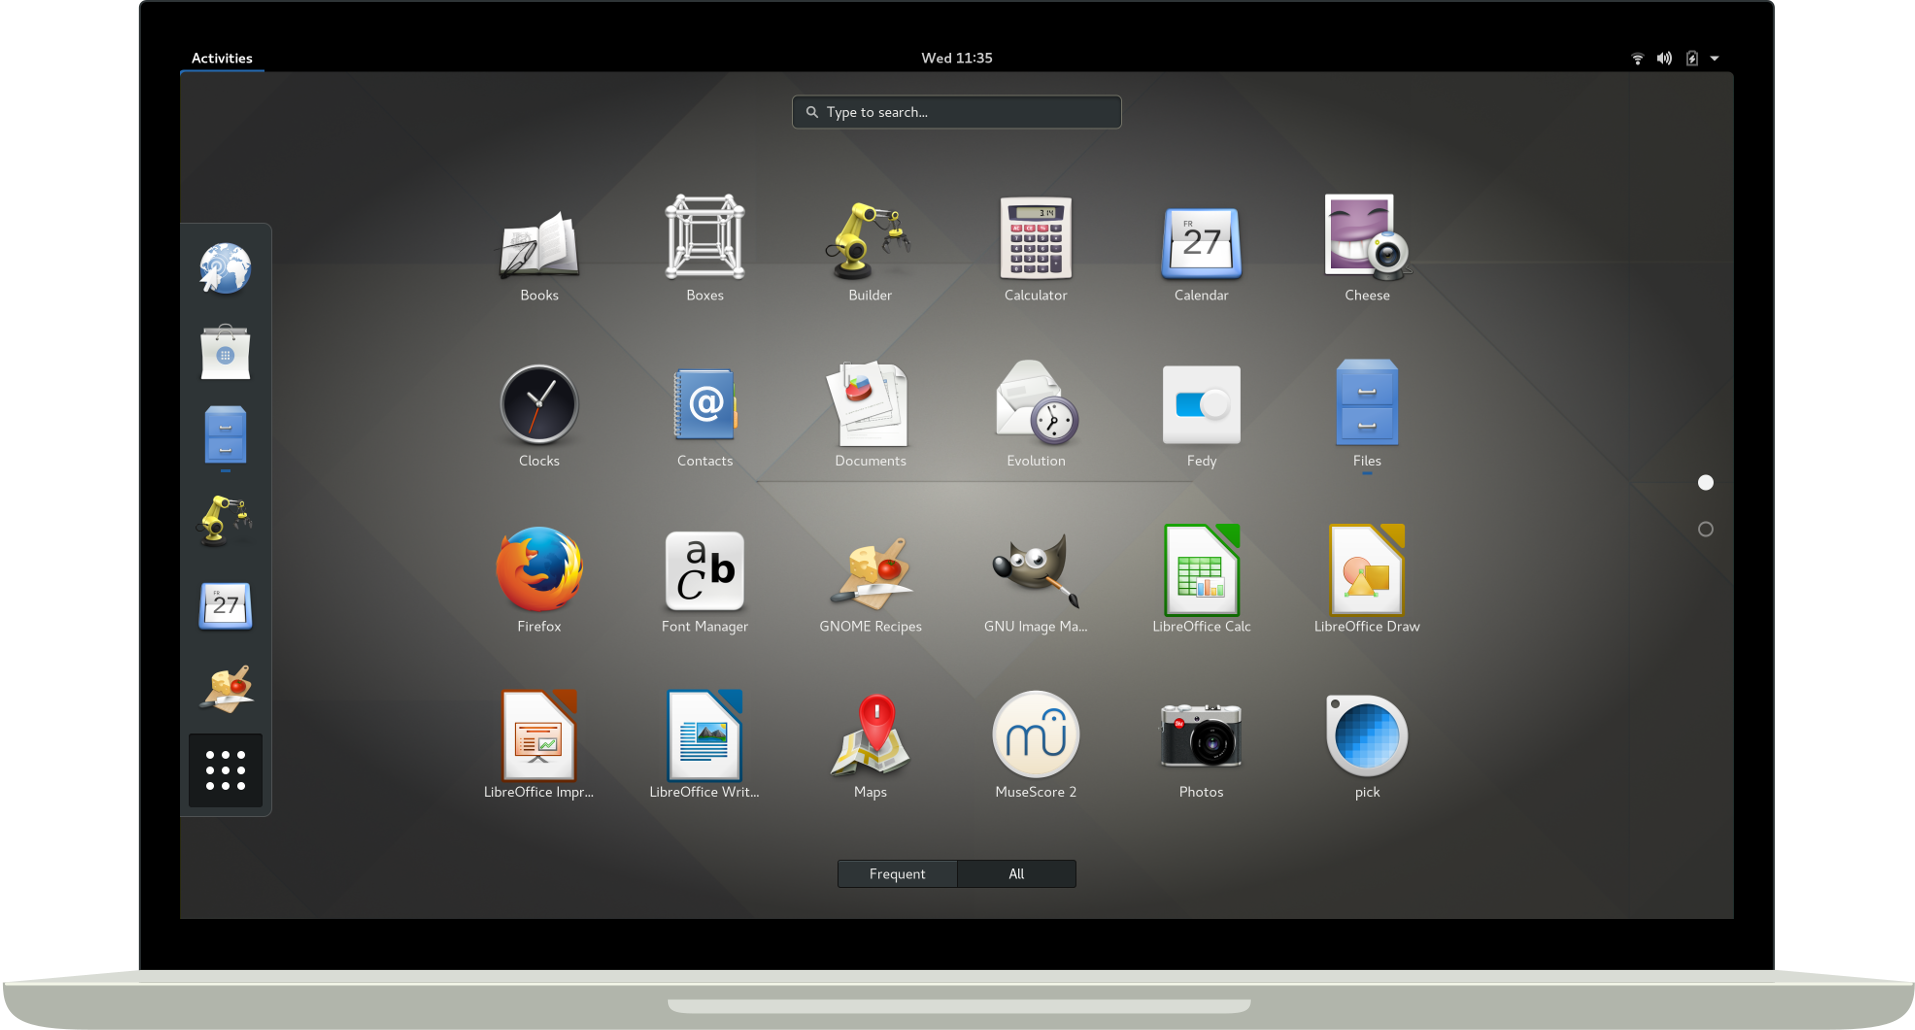
\includegraphics[scale=0.2]{images/GnomeScreen.png}
\end{frame}

\subsection{Présentation}
\begin{frame}
  \frametitle{Présentation}
  \begin{itemize}
  \item Environnement de bureaux
    \begin{itemize}
    \item Gestionnaire de fenêtres (Window Manager)
    \item Nombreux logiciels
      \begin{itemize} % CHECK
      \item Lecteur vidéo
      \item Visionneur d'image
      \item Navigateur de fichier
      \item etc.
      \end{itemize}
    \end{itemize}
  \item Utilisé dans de nombres système Linux
    \begin{itemize}
    \item Debian / Ubuntu
    \item Fedora / Red Hat
    \end{itemize}
  \item Actuellement en version 3.28
  \end{itemize}
\end{frame}

\subsection{Les outils collaboratifs}
\begin{frame}
  \frametitle{Les outils collaboratifs}
  
  %% Solution 1
  \begin{columns}
    \column{0.5\textwidth}
    \begin{itemize}
    \item Bugzilla
    \item Wiki GNOME
    \item Git (cgit/gitlab)
    \item \texttt{irc}
    \end{itemize}
    \column{0.5\textwidth}
    \begin{figure}
      
\includegraphics[scale=0.1]{images/bugzilla-logo.png} \\
      
\includegraphics[scale=0.04]{images/gnome-logo.png} \\
      
\includegraphics[scale=0.03]{images/git-logo.png}
      \hspace{0.1cm} 
\includegraphics[scale=0.03]{images/gitlab.png} \\
      
\includegraphics[scale=0.07]{images/irc-logo.png}
    \end{figure}
  \end{columns}

  %% %% Solution 2
  %% \begin{itemize}
  %% \item Bugzilla
  %% \item Wiki GNOME
  %% \item Git
  %% \item irc
  %% \end{itemize}
  %% \begin{figure}
  %%   
\includegraphics[scale=0.1]{images/bugzilla-logo.png} \hspace{1cm}
  %%   
\includegraphics[scale=0.04]{images/gnome-logo.png} \hspace{1cm}
  %%   
\includegraphics[scale=0.03]{images/git-logo.png} \hspace{1cm}
  %%   
\includegraphics[scale=0.07]{images/irc-logo.png}
  %% \end{figure}

  %% %% Solution 3
  %% \begin{itemize}
  %% \item Bugzilla
  %%   
\includegraphics[scale=0.1]{images/bugzilla-logo.png}
  %% \item GnomeWiki
  %%   
\includegraphics[scale=0.04]{images/gnome-logo.png}
  %% \item Git
  %%   
\includegraphics[scale=0.03]{images/git-logo.png}
  %% \item IRC
  %%   
\includegraphics[scale=0.07]{images/irc-logo.png}
  %% \end{itemize}
\end{frame}

\subsection{Newcomers}
\begin{frame}
  \frametitle{Newcomers}
  \begin{itemize}
  \item Outils pour les nouveaux contributeurs
    \begin{itemize}
    \item Builder
    \item Liste de projets
    \item Liste de bug simples
    \end{itemize}
  \item Canal de communication dédié
    \begin{itemize}
    \item Channel irc (\#newcomers)
    \item Mailing list
    \end{itemize}
  \end{itemize}
\end{frame}

\section{GNOME-Games}
\begin{frame}
  \frametitle{GNOME-Games}
  \includegraphics[scale=0.25]{images/screen-games.png}
\end{frame}

\subsection{Présentation}
\begin{frame}
  \frametitle{Présentation}
  \begin{itemize}
  \item Collection de jeux
    \begin{itemize}
    \item Jeux retro
    \item Natif Linux
    \end{itemize}
  \item Basé sur plusieurs bibliothèques
    \begin{itemize}
    \item libmanette
    \item retro-gtk
    \end{itemize}
  \end{itemize}
\end{frame}

\subsection{Contributions}
\begin{frame}
  \frametitle{Contributions - Documentation / Bug}
  \begin{itemize}
  \item Traçage d'un bug PulseAudio
    \begin{itemize}
      \item Problème complexe en apparence
    \end{itemize}
  \item Patch : Modifications du fichier 'HACKING'
    \begin{itemize}
    \item Utilisation de la syntaxe markdown
    \item Modification demandée par le mainteneur
    \end{itemize}
  \item Patch : Modifications du fichier 'README.md'
    \begin{itemize}
    \item Contribution à ``retro-gtk''
    \item Utilisation de la syntaxe markdown
    \end{itemize}
  \item Bug mannette XBox 360 (One)
    \begin{itemize}
    \item Impossible de configurer correctement le controller
    \item Gestion des boutons \texttt{LT2 RT2}
    \item Traçage et commentaire sur le bug
    \item Patch proposé par la communauté
    \end{itemize}
  \end{itemize}
\end{frame}

\begin{frame}
  \frametitle{Contributions - Code}
  \begin{itemize}
  \item Retour à la collection avec les touches \texttt{'Alt+Left'}
    \begin{itemize}
    \item Ajout d'une condition dans une fonction existant
    \end{itemize}
  \item Retour à la collection avec la souris
    \begin{itemize}
    \item Création d'une nouvelle fonction
    \item Nouveau signal capturé
    \item Problèmes rencontrés
      \begin{itemize}
      \item Environement de dev
      \item Documentation
      \end{itemize}
    \end{itemize}
  \item Correction de warnings dans \textit{retro-gtk}
  \end{itemize}
\end{frame}

\begin{frame}
  \frametitle{Contributions - Non réalisé}
  \begin{itemize}
  \item Conversion de Makefile à Meson
  \item Package Guix
  \item Implémentation de la suppression d'un élément de la collection
  \end{itemize}
\end{frame}


\subsection{Conclusion}
\begin{frame}
  \frametitle{Conclusion Games}
  \begin{itemize}
  \item Les outils collaboratifs
    \begin{itemize}
    \item Git 
    \item irc 
    \item Tracker de bug
    \end{itemize}
  \item Bilan du travaille effectué
  \end{itemize}
\end{frame}

\section{GNOME-Music}
\begin{frame}
  \frametitle{Le projet Gnome Music}
  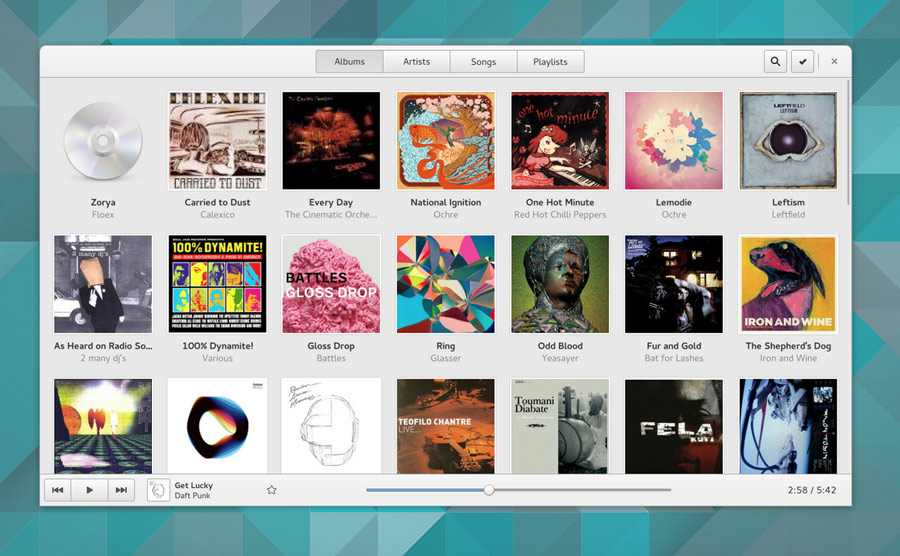
\includegraphics[scale=0.325]{images/gnome-music-app.png}
\end{frame}

\subsection{Contributions effectuées sur GNOME Music}
\begin{frame}
  \frametitle{Contributions effectuées}
  \begin{itemize}
  \item Rapport de bug sur le Builder
  \item Patch Pep8
  \item Patch Bouton retour arrière
  \item Patch Pep8 v2 + tox.ini
  \item Patch Album Cover Art
  
  \end{itemize}
\end{frame}

\subsection{Conclusion Music}
\begin{frame}
  \frametitle{Conclusion Music}
  \begin{itemize}
  \item Les acquis et difficultés
  \item La suite "perso"
  \end{itemize}
\end{frame}

\section{Conclusion}
\begin{frame}
  \frametitle{Conclusion}
  \begin{itemize}
  \item Bonne expérience
    \begin{itemize}
    \item Découverte de la contribution
    \item Sans doutes des contributions future
    \end{itemize}
  \end{itemize}
\end{frame}

\begin{frame}
  \frametitle{Questions ?}
\end{frame}

\end{document}
